\documentclass[a4paper,12pt,abstracton,titlepage]{scrartcl}
\usepackage{scrpage2}
\usepackage[utf8]{inputenc}
\usepackage[T1]{fontenc}
\usepackage[top=2.5cm, bottom=2.5cm, left=2cm, right=2cm]{geometry}
\usepackage[affil-it]{authblk}
\usepackage{lipsum}
\usepackage{url}
\usepackage[hidelinks]{hyperref}
\usepackage{graphicx}
\usepackage[table,xcdraw]{xcolor}
\usepackage{longtable}
\usepackage{multicol}
\usepackage{pdflscape}
\usepackage{listings}
\usepackage{caption}
\usepackage{float}
\usepackage[export]{adjustbox}

%citations
\usepackage{multibib}
\newcites{ac}{Academic references}
\newcites{nac}{Informal references}

% code for generating glossary, from http://tex.stackexchange.com/a/5837/59718
\usepackage[acronym,toc]{glossaries}
\usepackage{glossary-mcols}
\newcommand{\dict}[2]{%
  \newglossaryentry{#1}{name=#1,description={#2}}%
  \glslink{#1}{}%
}
\makeglossaries

% Here we set up the header, meta-information and front matter
%\date{December 16, 2014}      %// Today's date will appear when this is commented out.
\newcommand{\version}{0.1}

% title page
\author{Daniel S. C. Schiavini and Maarten Baertsoen}
\affil{Open Universiteit Nederland, faculteit Informatica \\
	T61327 - Afstudeerproject bachelor informatica}
\title{Project Documentation}
\subtitle{Useful feedback in the Ampersand parser\\
	~\\
	Phase 3d}
\publishers{Version \version}

% header
\pagestyle{scrheadings}
\setheadsepline{0.2pt}
\clearscrheadings
\automark[section]{chapter}
\ihead{Daniel S.C. Schiavini and Maarten Baertsoen}
\ohead{Ampersand Parser: Project documentation}
\cfoot{\pagemark}

% URL's
\renewcommand*{\UrlFont}{\footnotesize\ttfamily}

% hyphenation 
\hyphenation{
	gua-ran-tee
	pro-duct
	cor-res-pon-ding
	me-cha-nism
  ma-nu-al-ly
	know-ledge
	de-ve-lo-pers
	do-cu-men-ta-tion
  un-ne-ces-sa-ry
	sa-tis-fac-tion
	Schi-a-vi-ni
	Ba-ert-so-en}

% Now the document starts
\begin{document}
\maketitle
\newpage

\tableofcontents
\listoffigures
\listoftables
\clearpage

% !TEX root = ../Documentation.tex
\section{Introduction}
\subsection{Identification}
This document contains the domain \& techniques analysis of the project `Useful feedback in the Ampersand parser'.
The document is the milestone product of the project phase 3a for Daniel S.C. Schiavini, as specified in the project planning \citenac{plan}.

This document is part of the graduation project of the computer science bachelor at the Open Universiteit Nederland.
The project `Useful feedback in the Ampersand parser' is executed in collaboration with Maarten Baertsoen, with support of the supervisor Dr. Bastiaan Heeren and examiner Prof.dr. Marko C.J.D. van Eekelen.
The assignment is given by Prof.dr. Stef Joosten, who researches how to further automate the design of business processes and information systems by the development of the Ampersand project.

Ampersand is an approach for the use of business rules to define the business processes.
Users describe the business rules in a formal language (ADL), and Ampersand compiles those rules into functional specification, documentation and working software
prototypes.
The main objective of this project is to improve the feedback and maintainability of the Ampersand parser.
See \citenac{plan} for more details on the project.

\subsection{Goals}
\lipsum[3]

\subsection{Document overview}
\lipsum[4]
% !TEX root = ../Documentation.tex

\section{Analysis}
\label{sec:analysis}
In this section, we analyze the previous Ampersand parser in order to understand its workings and signal the improvement points.

\subsection{System overview (R-M)}
The requirements of the new parser have been described in the project planning \citenac{plan}.
Basically, both the old and the new parser must be able to make a conversion from a text file (ADL-script) to a parse tree (the P-structure).
\autoref{fig:data-flow-1} depicts this data flow.
%
\begin{figure}[htb!]
	\centering
	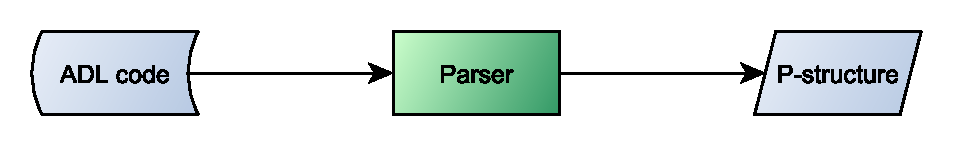
\includegraphics[width=0.586\textwidth]{Figures/DataFlow1}
	\caption{Relevant data flow for the Ampersand parsing component}
	\label{fig:data-flow-1}
\end{figure}

Often, the parsing component is separated into a lexer (that converts text to tokens) and the actual parser (that converts the tokens into the parse tree).
Since this separation is considered beneficial for both maintainability and performance \citeac{parsec}, we assumed from the beginning that the new Ampersand parser would be separated in this way.
This is depicted in \autoref{fig:data-flow-2}.
The previous parser also had a separate lexer, but the name was scanner instead.
%
\begin{figure}[htb!]
	\centering
	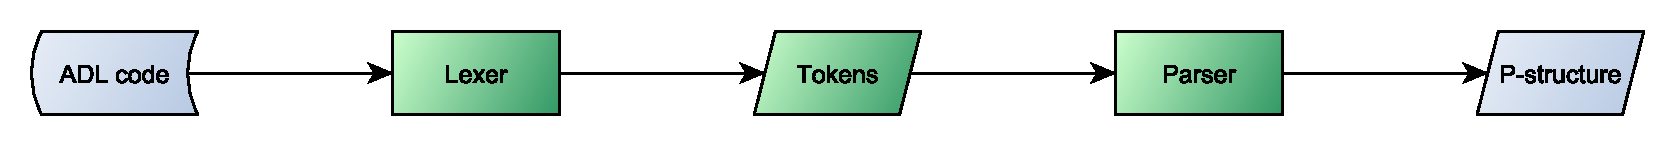
\includegraphics[width=1\textwidth]{Figures/DataFlow2}
	\caption{Data flow for the Ampersand lexing and parsing components}
	\label{fig:data-flow-2}
\end{figure}

In order to take the next steps and understand how the parser can be designed, we first take a look at the grammar in \autoref{subsec:analysis-grammar} and the parse tree in \autoref{subsec:analysis-parse-tree}.
Afterwards, we analyze the lexer with the original token structure, so that we can define a new token structure, in \autoref{subsec:analysis-lexer}.
Finally, we analyze the parser in \autoref{subsec:analysis-parser} and the generated errors in \autoref{subsec:analysis-errors}.

\subsection{Grammar (M)}
\label{subsec:analysis-grammar}
\dict{EBNF}{Extended Backus-Naur Form}%
\dict{Extended Backus-Naur Form}{Notation technique for documenting context-free grammars}%

\subsection{Getting the EBNF in good shape}
The Ampersand syntax is described using the EBNF notation. 
At the beginning of the project, we noticed that the existing EBNF diagram was not in line anymore with the actual syntax of Ampersand.
As the EBNF is a crucial source of information in building the new parser, the first focus was to update the old EBNF to represent the actual Ampersand Syntax.

Through reverse engineering, we checked all Haskell functions on the actual syntax they implement.
In the source of the new parser, all the syntax notations are placed above the actual parser function to support code maintainability.

The derived, and up to date, syntax is visualized using a railroad diagram, an ideal technique to visualize context free grammars.
Several railroad diagram generators are available on the internet, free of charge.
We used the railroad diagram generator created by Gunter Rademacher, available on http://bottlecaps.de/rr/ui.
During the actual generation, the generator failed on the Ampersand Syntax, more precisely on the statement: Exp4 ::= Exp5 (( ';' Exp5 )* | ('!' Exp5)*)
Convinced of the correctness of the EBNF statement, we contacted the owner of the tool, and he discovered a bug in his tool which he corrected promptly.

\subsection{The actual EBNF diagram}

TODO: Show/describe the EBNF (maybe actual EBNF as attachment).
TODO: Note that this EBNF was not available, but we had to derive it from the parser.
TODO: Note that we helped the railroad site to resolve a bug.

One interesting plus is that during the project we found a bug in the Railroad Diagram Generator.
The tool would crash with the \hyperref[fig:ebnf-Trm4]{\texttt{Trm4}} expressions.
This bug was reported to the author Gunther Rademacher, who promptly fixed the issue.

\subsection{Parse tree (R-M)}
\label{subsec:analysis-parse-tree}
The parse tree (also known as P-structure) is a data structure that very much resembles the EBNF description.
The root of the tree is the \texttt{P\_Context} structure, and every leaf of the tree has a field for the location where it was found in the ADL code (the \texttt{Origin} structure).
The tree is consistently defined with the record syntax and is well documented.

However, the constructions are not completely pure, since some transformations are necessary from the ADL to the P-structure.
This forces the parser to do more than only parsing.
Also, the order of the fields can be confusing; sometimes \texttt{Origin} is the first field and sometimes it is not.

During this project, small changes to the parse tree have been done.
These changes are described in \autoref{subsec:design-parse-tree}.

\subsection{Lexer (M)}
\label{subsec:analysis-lexer}
TODO: describe the possible improvements in the old lexer.

\subsubsection{Token structure}
TODO: Describe the old token strucure

\subsubsection{New token structure}
TODO: Develop a better token structure

\subsection{Parser (R-M)}
\label{subsec:analysis-parser}
The previous Ampersand parser was generally well organized, so each ENBF rule could be mapped to a different parser.
However, several flaws were observed as improvement points.
During this project, we focused on the following issues:
\begin{description}
  \item[Lacking documentation]
    There was no documentation on the recognized grammar.
    The last EBNF available was not updated in a long while.
  
  \item[Ad-hoc transformations]
    The parser was built with the applicative interface of the uulib.
    The applicative operators were thus used in sequence to recognize each of the accepted grammar productions.
    However, the parser was often forced to change the order and format of the parsed structures, because the parse tree did not match the grammar productions (i.e. many rebuild functions).
    
  \item[Long file]
    Since all the grammar constructions -- plus help functions -- were in a single file, the parser was hardly readable.
    It summed a total of 823 lines of code only in the \texttt{Parser} module.
  
  \item[Pretty printing]
    It used to be impossible to print the parse tree back to ADL-code.
    That made it harder to develop and test the parser properly.
  
  \item[Test suite]
    There were no automated tests for the parser.
    Because of this, any code change would be hard to test and could potentially influence other Ampersand modules.
  
  \item[Duplicated code]
    A large part of the code was duplicated and not used (mainly in the \texttt{Parsing} module).
  
  \item[Error messages]
    As mentioned, the main reason for this project was the bad quality of the error messages generated.
    \autoref{subsec:analysis-errors} expands on this point.
\end{description}
%
Although it may be hard to resolve all the mentioned issues, we believe our efforts have played off well.
In \autoref{subsec:design-parser} we describe how the new parser was designed.

\subsection{Errors (M)}
\label{subsec:analysis-errors}
TODO: show how the parser did not provide good errors, and how we could improve them.

% !TEX root = ../Documentation.tex

\section{Design}
\label{sec:design}

\subsection{System overview (D)}
  The parser module overview is given in \autoref{fig:ParserModules}.
  Each of the modules are described in the following subsection.
  %
  \begin{figure}[ht]%
    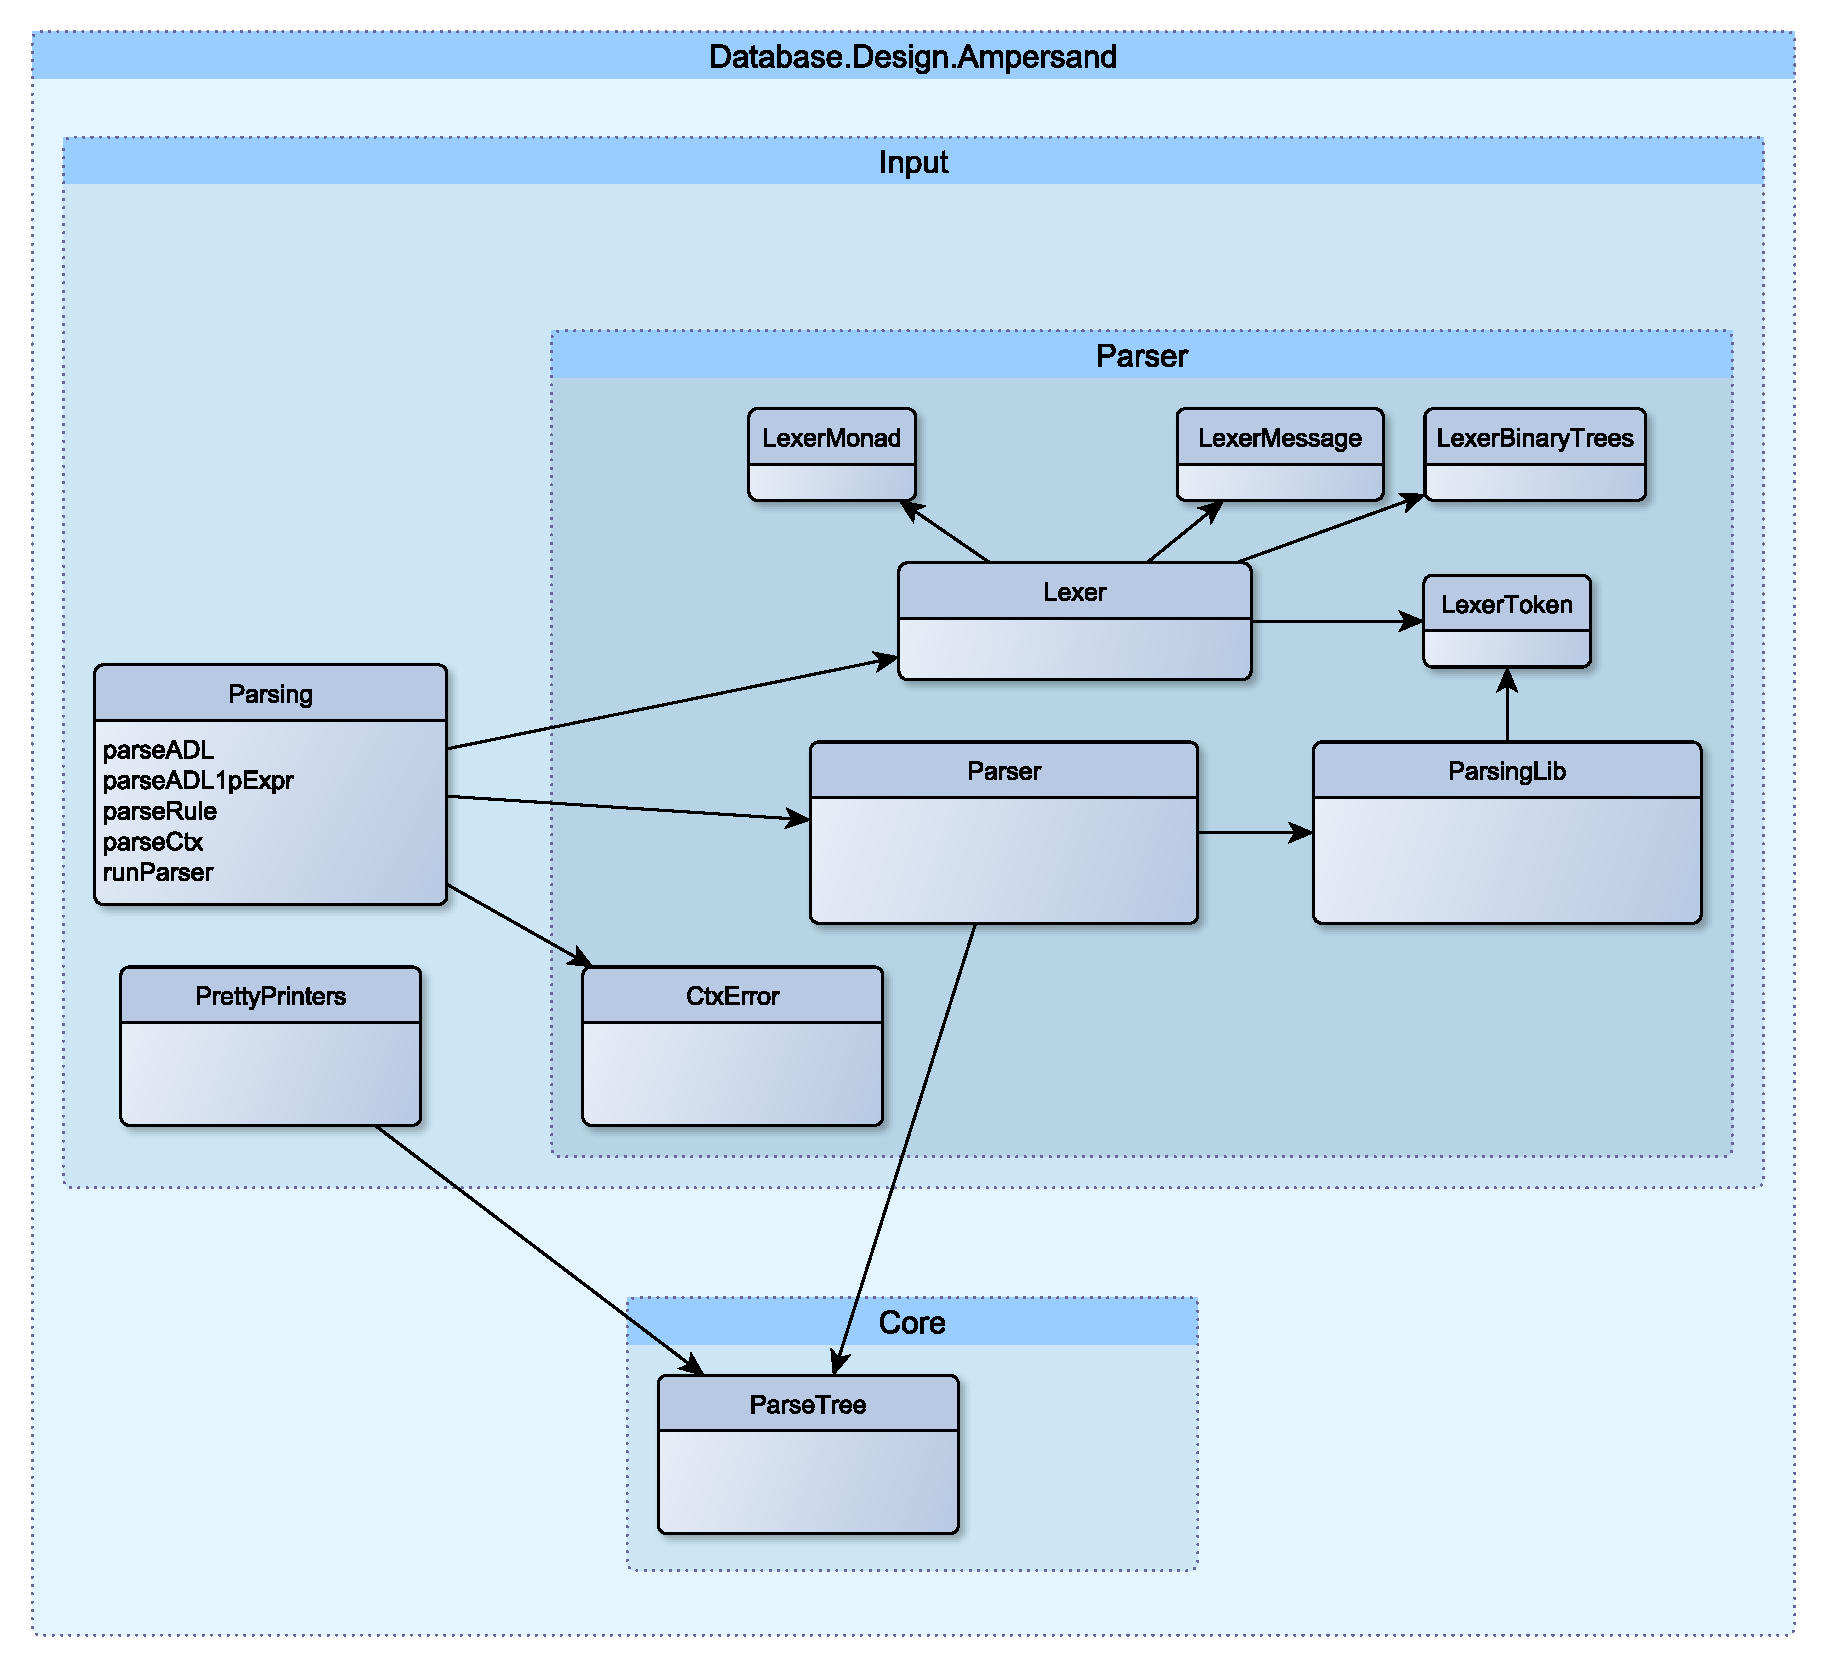
\includegraphics[width=\columnwidth]{Figures/ParserModules}
    \caption{The parser modules and their relationships}
    \label{fig:ParserModules}
  \end{figure}%
  TODO: Add the exported functions to each module.

  \subsubsection{Modules}
  \label{subsec:parser-modules}
  In this section a short description of each module is given:
  %
  \begin{description}
    \item[Parsing] module that implements the interface of the parser with the rest of the system.
      It is responsible for reading the input files, calling the lexer and the parser and returning a parse tree as result (or a parse error).

    \item[Parser] module responsible for executing the parsing itself.
      It accepts the tokens that are allowed in each grammar production and generates the corresponding parse tree.
      The parser is described in \autoref{subsec:design-parser}.
      
    \item[ParsingLib] library that contains several useful functions to assist the parser, e.g. token recognition.
      These functions are not depending on the specific grammar rules.
      
    \item[ParseTree] external module containing the parse tree data structures.
      Only details of this module have been changed during this project (e.g. field ordering).
    
    \item[PrettyPrinters] contains the \texttt{Pretty} class and the functions responsible for printing the parse tree to ADL scripts in a `pretty' way.
    
    \item[CtxError] contains the data structures responsible for the parse errors and their location.
      This module has not been refactored as a part of this project.
    
    \item[Lexer] module responsible for recognizing the input characters and converting them to tokens.
      The lexer, together with its sub-modules, is described in \autoref{subsec:lexer}.
  \end{description}

\subsection{Lexer (M)}
\label{subsec:lexer}
The lexer module is responsible to split up the input stream into tokens.
Tokens are meaningful pieces of the input strings that needs to be kept together together.

\subsubsection{The rationale behind the new lexer}
In the design of the new Ampersand parser, the question arose whether to keep the current scanner or to implement a new one.
After the analysis of the error improvement areas, the main improvements were identified within the actual parser.
The error feedback quality produced by the scanner module was higher and therefore, there was no stringent need to re-implement the scanner.
On the other hand, given the aspect that Parsec was defined as the new Parser library, keeping the current scanner would have resulted in the utilization of 2 different libraries providing more of less the same functionality.
To avoid a decrease in maintainability, the decision is made to implement the parser and scanner based on the same library.
During the implementation of the lexer module, replacing the old scanner, additional attention was given to further improve the quality of the error messages
The scanner module is renamed to the lexer module to stress the aspect that the principle of lexemes is used in the new scanner.

The lexer is build based on the existing Helium lexer modules. 
One of the main goals of this project create a compiler and a dialect of Haskell in which clear error messages were produced. TODO: reference
The Lexer module in Helium contains interesting principles such as position monitoring, warnings and easy maintainable error messages.


\subsubsection{Lexer structure}


The lexer is the main module, in which the actual lexing is done, and to do so, it it using the following sub-modules:

 \begin{description}
 
    \item[LexerMonad] contains a monad definition that supports lexing with context.
      It tracks for example the location in the input and the warnings that may be generated.
	  This module is re-used without any modification out of the  Helium parser.
      The following functions or types are used in the Ampersand lexer:
	  \begin{itemize}
		\item [LexerMonad] is the main monadic type used in the lexer returning an error or a list of tokens together with a list of warnings
		\item [addPos] is used to trace the position of the token
		\item [lexerError] to generate lexer error
		\item [lexerWarning] to generate lexer warnings
		\item [runLexerMonad] main function to handle the LexerMonad results 
	  \end{itemize}
	  
    \item[LexerMessage] contains functions to handle errors and warnings from the lexer.
	  Based on the warning/error type and the needed language, LexerMessage will fetch the correct description of an error or a warning out of the LexerTexts module
	  The show functions for the error and warning are maintained in this module.
	  
    \item[LexerTexts] will fetch the correct description of an error or a warning out of the LexerTexts module.
	  This centralisation provides an easy entry point for the maintenance of the actual messages as the actual messages are no longer dispersed over the module functions.
	  
    \item[LexerBinaryTrees] module responsible for searching binary trees in an efficient way, to support the token recognition.
            This is the existing UU_BinaryTrees module which is renamed to match the used naming structure of the new lexer modules.

    \item[LexerToken] contains the data structure, and corresponding show function, that represents the input tokens for the lexer.
	
  \end{description}

Each token contains a part of the input string together with an identifier, defining the token content, and the position of the token in the input file.
The token structure is defined as follows:

data Token = Tok \{	  tokLex :: Lexeme
                		, tokPos :: FilePos \}

The lexeme is the combination of the token type and the actual token content, sliced from the input string.
FilePos is used to keep track of the original position of the lexeme in the input string.

During the lexer processing, the input file is processed sequentially.
All kind of differentiating formats are checked in a specific order, and each time a match is found, the lexeme is extracted from the input file and the token is created.
In the token creation, function ReturnToken, the position and lexeme is grouped into the actual token and the next nested lexer iteration is launched.


\subsection{Parser (R-M)}
\label{subsec:design-parser}
The mainstream design of the new parser has not changed much.
Basically, each EBNF rule receives its own parser function.
Thanks to the combinator operators, each parsing function also looks very similar to its corresponding EBNF.

The applicative interface is consistently used.
By changing details of the implementation, e.g. the order of the fields in the parse tree, we have made many of the `rebuild' functions unnecessary.
For some parsers the amount of changes necessary in order to remove supporting functions was too large or even impossible with the current parse tree.

Note that in parts of the parser, the function syntax has substituted the record syntax for creating data objects.
This was done only when the code readability could be improved by doing so.

\subsubsection{Parsec}
\label{subsec:design-parsing-lib}
As mentioned earlier, and described in research context document \citenac{parsing}, the new Ampersand parser has been rebuilt with another parsing library, namely Parsec.
However, for the Ampersand developers, the source code of the parser will still look very familiar, thanks to the applicative interface.
For developers, the main differences between Parsec and the uulib are:
\begin{itemize}
  \item Parsec does not backtrack by default.
    In order to enable backtracking, the \texttt{try} function must be used.
    This is described in \autoref{subsec:backtracking}.
  \item Parsec does not try to solve parsing errors.
    The parser stops immediately after the first issue.
    See also the error analysis in \autoref{subsec:design-errors}.
  \item Error messages are customizable by using the \texttt{<?>} operator.
    This is also suggested in \autoref{subsec:design-next-steps}.
  \item Some combinators have a different name, e.g. one must use \texttt{option} instead of \texttt{opt}.
    Assuming the documentation found on Hackage is clear and sufficient, interface differences are not documented here.
\end{itemize}

\subsubsection{Backtracking}
\label{subsec:backtracking}
In order to explain the differences on backtracking behavior between the uulib and Parsec, we quote here Doaitse Swierstra, the author of the uulib \citenac{swierstra-parsec}:
\begin{quote}
\textsl{To understand the subtleties it is important to understand the differences between the try construct in Haskell and the non-greedy parsing strategy used in uu-parsinglib. Effectively the latter is a try which just looks ahead one symbol. In that respect it is less powerful than the try construct from Parsec, in which you specify that a specific construct has to be present completely. And then there is the underlying different overall strategy. Parsec uses a back-tracking strategy with explicit tries to commit, whereas uu-parsinglib uses a breadth-first strategy with an occasional single symbol look-ahead.}
\end{quote}
%
We can therefore conclude that the try-statements in Parsec are undesirable.
However, they are necessary when the grammar is ambiguous.
In this section we explain why each of the remaining try statements are necessary, and how these issues can be resolved:
\begin{description}
  \item[Classify]
    This ambiguity in the grammar arises from the \texttt{Classify} and \texttt{GenDef} productions:
    \begin{quote}
        \texttt{Classify ::= `CLASSIFY' ConceptRef `IS' Cterm}\\
        \texttt{GenDef ::= (`CLASSIFY' | `SPEC') ConceptRef `ISA' ConceptRef}
    \end{quote}
    When the parser encounters \texttt{`CLASSIFY'}, it cannot define whether it found a \texttt{Classify} or a \texttt{GenDef} production.
    Therefore, the parser must consume the keyword and a \texttt{ConceptRef} before consuming either \texttt{`IS'} or \texttt{`ISA'} and determining which production is applicable.
    
    In order to solve this issue, one must choose a different keyword or symbol for each of the productions.
    Another option would be to merge the two statements in the same parser.
    We did not merge the productions because that would make the parser less maintainable.
  
  \item[Role]
    This ambiguity in the grammar arises from the \texttt{RoleRelation} and \texttt{RoleRule} productions:
    \begin{quote}
        \texttt{RoleRelation ::= `ROLE' RoleList `EDITS' NamedRelList}\\
        \texttt{RoleRule ::= `ROLE' RoleList `MAINTAINS' ADLidList}
    \end{quote}
    When the parser encounters \texttt{`ROLE'}, it cannot define whether it is a \texttt{RoleRelation} or a \texttt{RoleRule} production.
    Therefore, the parser must consume the keyword and a \texttt{RoleList} (which may be long) before consuming either \texttt{`MAINTAINS'} or \texttt{`EDITS'} and determining which production is applicable.
    
    In order to solve this issue, one must choose a different keyword for each of the productions, merge the two options to have the same representation in the parse tree, or refactor the parser so that the two options are parsed together.
    We did not merge the productions because that would make the parser less maintainable.
  
  \item[View]
    This ambiguity in the grammar arises from the \texttt{FancyViewDef} and \texttt{ViewDefLegacy} productions:
    \begin{quote}
        \texttt{FancyViewDef ::= `VIEW' Label ConceptOneRefPos `DEFAULT'? `\{' ViewObjList `\}' HtmlView? `ENDVIEW'}\\
        \texttt{ViewDefLegacy ::= (`VIEW' | `KEY') LabelProps ConceptOneRefPos `(' ViewSegmentList `)' }
    \end{quote}
    When the parser encounters \texttt{`VIEW'}, it cannot define whether it found a \texttt{FancyViewDef} or a \texttt{ViewDefLegacy} production.
    In this case, defining which construction is applicable is even more complicated.
    This decision must, in the worst case, be delayed until the parser encounters a \texttt{`\{'} or \texttt{'('}.
    That's because the productions \texttt{Label} and \texttt{LabelProps} are not disjoint, and \texttt{`DEFAULT'} is optional.
    
    In order to solve this issue, we advise to merge or drop the legacy statement.
    
  \item[Multiplicity]
    This ambiguity in the grammar arises from the \texttt{Mult} production:
    \begin{quote}
        \texttt{Mult ::= (`0' | `1') `..' (`1' | `*') | `*' | `1'}
    \end{quote}
    When the parser encounters \texttt{`1'}, it cannot define whether it found the first or the last production.
    The parser must therefore read the next token before choosing the right option.
    
    In order to solve this issue, we advise to refactor the grammar (and the parser) to have the following production:
    \begin{quote}
        \texttt{Mult ::= `0' `..' (`1' | `*') | `1'(`..' (`1' | `*'))? | `*'}
    \end{quote}
    %
    We did not refactor the code in this matter because the \texttt{pMult} parser does more than only parsing: it also changes the representation of the found constructions before creating the parse tree.
  
  \item[Labels and Terms]
    In the productions \texttt{IndAtt}, \texttt{ViewAtt} and \texttt{RuleDef}, we see very similar ambiguities:
    \begin{quote}
        \texttt{IndAtt ::= LabelProps? Term}\\
        \texttt{ViewAtt ::= LabelProps? Term}\\
        \texttt{RuleDef ::= `RULE' Label? Rule Meaning* Message* Violation?}
    \end{quote}
    Wherein:
    \begin{quote}
        \texttt{Label ::= ADLid ':'}\\
        \texttt{LabelProps ::= ADLid (`{' ADLidListList `}')? `:'}\\
        \texttt{Rule ::= Term ('=' Term | '|-' Term)?}
    \end{quote}
    And one of the possible productions of \texttt{Term} is:
    \begin{quote}
        \texttt{Term ::= Trm2 ::= Trm3 ::= Trm4 ::= Trm5 ::= Trm6 ::= RelationRef ::= NamedRel ::= Varid Sign?}
    \end{quote}
    While:
    \begin{quote}
        \texttt{ADLid ::= Varid | Conid | String}
    \end{quote}
    
    What happens here is that when the parser encounters a \texttt{Varid}, it cannot define whether it is part of the (optional) \texttt{Label} production or if no \texttt{Label} was given and the \texttt{Varid} is part of a \texttt{Term}/\texttt{NamedRel} production.
    
    Due to the quite complex grammar for the \texttt{Term} production, this issue may severely impact the parser's performance.
    This is probably the most harmful of the ambiguities mentioned.
    However, it can only be solved by adding a symbol before the \texttt{Term} production (e.g. making the `:' non-optional).
    
    \textbf{TODO: IndAtt and ViewAtt are the same parser.}
\end{description}
%
Please note that in order to have proper backtracking with correct error messages, Parsec may require two try-statements \citenac{try-harmful}.

\subsection{Parse tree (R-M)}
\label{subsec:design-parse-tree}
Improvements in the Ampersand parse tree are out of the scope of this project, because of the potential consequences to the rest of the Ampersand system.
However, during the development of the new parser a few constructions have been changed in order to make the parser more readable and maintainable.
The changes have been mostly in the order of the constructor parameters, and this was done consequently though all Ampersand modules.
The updated parse tree is depicted in the appendices (\autoref{fig:parse-tree}).

\subsection{Errors (M)}
\label{subsec:design-errors}
TODO: show what we've done to improve the errors.

\subsection{Next steps (M)}
\label{subsec:design-next-steps}
TODO: give tips on how to further improve the parser. e.g.:
  - cleanup CtxError, add warnings, use <?> for the errors.
  - reorganize parse tree, e.g. using always Origin as first parameter.
% !TEX root = ../Documentation.tex

\section{Test Report}
\label{sec:tests}

\subsection{Test suite}
  Together with the new parser, a test suite has been developed.
  This test suite has been used to verify the performance and correctness of the new parser.
  The source code can be found in the folder \texttt{src/Database/Design/Ampersand/Test} within the Ampersand repository.

  The test suite runs in three steps, which are depicted in \autoref{fig:TestModules}.
  Each of the modules are described in the following subsection.
  %
  \begin{figure}[ht]%
    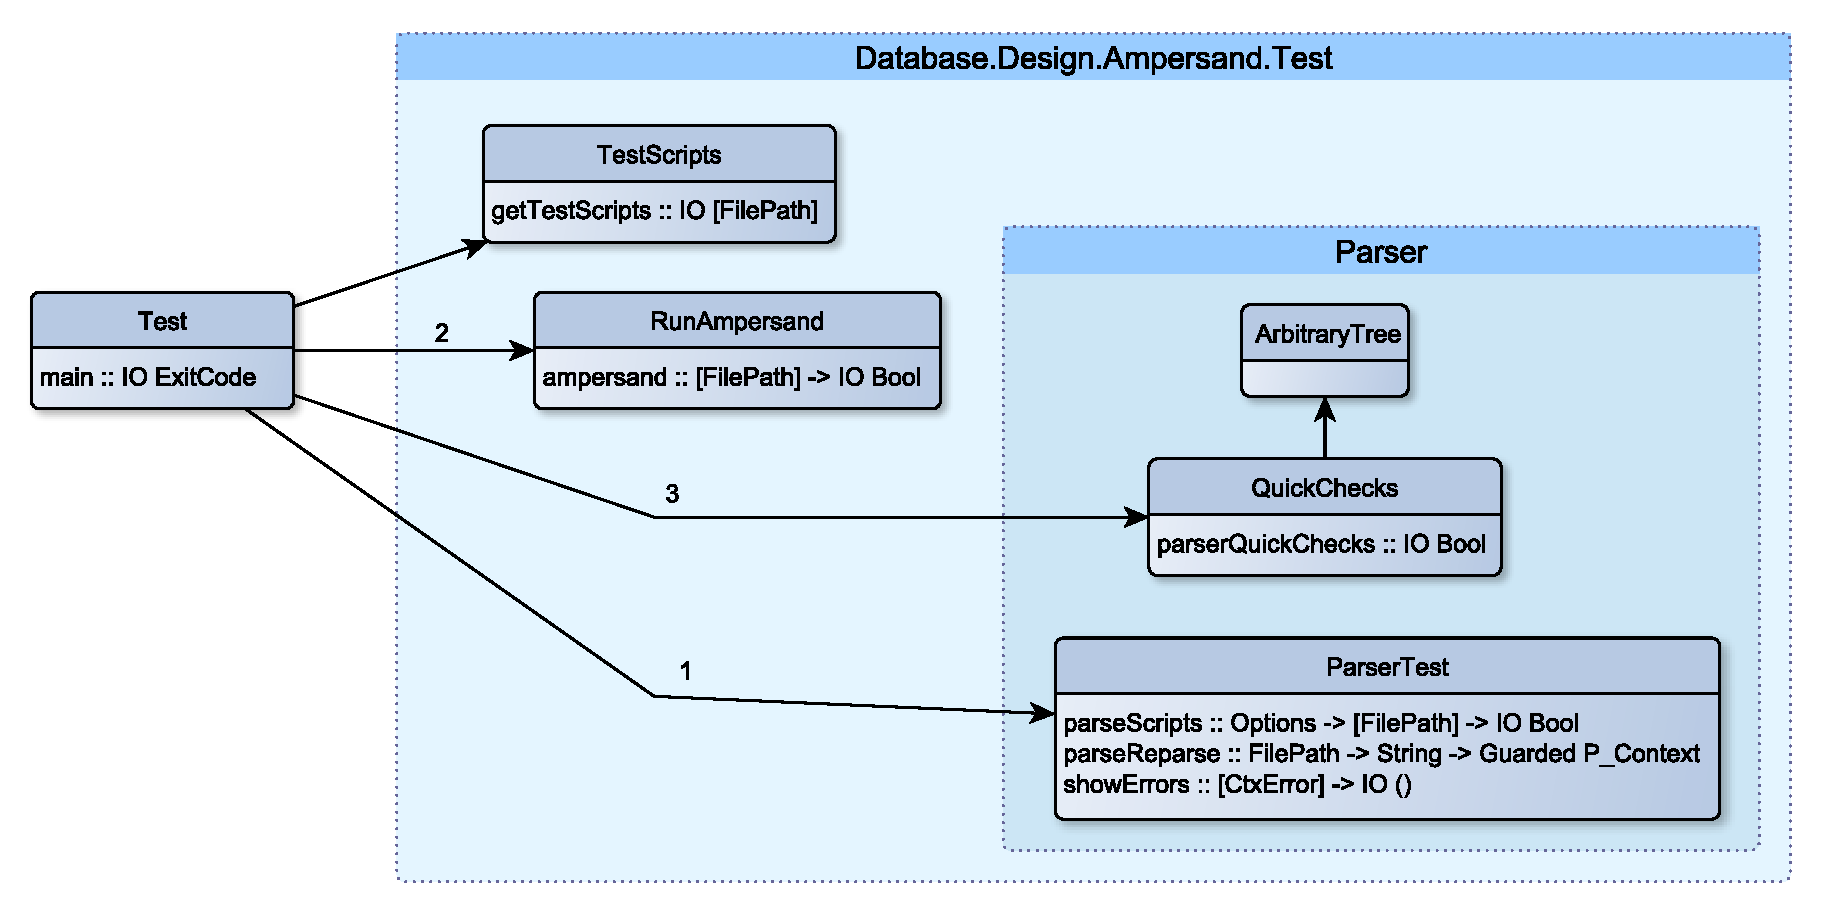
\includegraphics[width=\columnwidth]{Figures/TestModules}
    \caption{Test suite modules with their exported functions}
    \label{fig:TestModules}
  \end{figure}%

  \subsubsection{Modules}
  \label{subsec:test-modules}
  In this section a short description of each module is given:%
  %
  \begin{description}
    \item[Test] contains the \texttt{main} method that can be executed to run the test suite.
      The \texttt{main} function calls each of the other modules in sequence, stopping if any of them returns \texttt{False}.
      When all tests have been successful, the return code is \texttt{ExitSuccess}.
      Otherwise, the return code is naturally \texttt{ExitFailure}.
    
    \item[TestScripts] retrieves a list of scripts that can be used for the different tests.
      It searches for tests within the folder \texttt{ArchitectureAndDesign}, and contains a list of scripts from the \texttt{ampersand-models} repository, that can be changed at a later moment if wished.
      Note that all the ADL-scripts listed in this section must be correct for the parser and the type checker.
    
    \item[ParserTest] exports three functions that are the core of testing the parser:
      \begin{itemize}
        \item \texttt{parseScripts} receives a list of files to parse, and checks that every file can be parsed successfully.
        \item \texttt{parseReparse} tries to parse a file, and if sucessfull, pretty-prints the result and parses it again.
        \item \texttt{showErrors} prints the given parse errors to the output.
      \end{itemize}
    
    \item[RunAmpersand] receives a list of files, and checks that every file can be executed successfully by Ampersand.
      This tests thus not only the parser, but also the interface between the parser and the type checker, as the rest of the Ampersand chain.
    
    \item[QuickChecks] generates random parse tree structures and generates the corresponding ADL-script by pretty printing the parse tree.
      This ADL-script is then fed back to the parser through the \texttt{parseReparse} function, to verify that the parser can accept any random input.
      More information on the quick checks is given in subsection~\ref{subsec:quick-check}.
    
    \item[ArbitraryTree] is a support module that gives \texttt{Arbitrary} instances to all parse-tree structures.
      This is used by QuickCheck as described in subsection~\ref{subsec:quick-check}.
    
    \item[ArbitraryPandoc] contains \texttt{Arbitrary} instances to the Pandoc data types.
      This file has not been developed in this project, but copied from the \texttt{jgm/pandoc} project with the GPL license.
  \end{description}

  \subsubsection{QuickCheck and pretty printing}
  \label{subsec:quick-check}
  The most innovative part of the test suite is the use of random structures to test the parser.
  In this section we describe how this generation is implemented.
  
  The main role in the generation of random structures is played by the support library QuickCheck, which has been added to the Ampersand project.
  QuickCheck is able to generate any data structure randomly.
  However, since the parse tree is a custom structure that must obey specific rules, QuickCheck requires the specification of these rules by instances of the \texttt{Arbitrary} class.
  
  Every data structure in the parse tree has received an \texttt{Arbitrary} instance used for test purposes.
  The instances can be found in the module \texttt{Database.Design.Ampersand.Test.Parser\-.ArbitraryTree}, as described in subsection~\ref{subsec:test-modules}.
  
  After generating the random parse trees, the test suite needs to convert them to ADL-scripts.
  The conversion of parse tree to source code is also known as pretty printing.
  As the pretty printing is seen as part of the parse tree, it is not included in the Test modules, but is part of the input subsystem.
  The pretty printing instances are found in the module \texttt{Database.Design.Ampersand.ADL1.PrettyPrinters}.
  This module makes use of the library \texttt{Text.PrettyPrint.Leijen}, that outlines the output so it is indeed `pretty'.
  
  Now that the ADL source is available, the parser is executed.
  The result of the parser is checked to be equal to the generated tree by the property \texttt{prop\_pretty}.
  The property is currently tested for 64 generated parse trees in the test suite.
  If the test fails for any generated structure, the test suite fails with an appropriate error.
  
  \subsubsection{Running the tests}
  During the parser development, the \texttt{main} function of the parser tests has been executed manually, through a batch file.
  This is mainly done because the project team did not have access to the Sentinel server, and no documentation was available on how to run Sentinel locally in a Windows machine.
  However, now that the parser is being delivered, it should be integrated with the other existing Ampersand/Sentinel tests.
  We leave the option open for the Ampersand development team to either add the Sentinel jobs to this test suite, or to add the parser test suite to the Sentinel jobs.
  
\subsection{Errors}
  Since evaluating the quality of error messages is manual work, the errors have not been included in the test suite.
  TODO: Give Maarten's findings on how the errors have improved. Maybe the tables should be an attachment, but the summary should be here.

\subsection{Next steps}
  In this section we name a couple changes that can be done in the test suite in the future:
  \begin{description}
    \item[Sentinel] During the development of the new parser, we worked in a separate fork.
      Our changes were not being tested in the Ampersand test server (Sentinel).
      Since we did not have access to this server, we developed a separate test suite.
      It may be pertinent to integrate the Sentinel jobs into the test suite or to integrate the test suite into the Sentinel jobs.
    
    \item[Output] Currently, the test suite outputs errors by using the \texttt{Debug.Trace} module.
      From a purely functional perspective, using this module may be undesirable.
      Therefore, the Ampersand team may consider changing the test outputs to use IO with monads in a more functional way.
  \end{description}


\newpage
% !TEX root = ../Parsing.tex

\section{Conclusion}
\label{sec:conclusion}
In \autoref{sec:libraries}, the advice was given to use a combinator library for the new parser of Ampersand.
The main reason to avoid the parser generators is that it is hard to generate useful feedback.
Then, in \autoref{sec:errors}, it was made even more clear that besides generating good messages, those messages should also be customizable.

Therefore, the advice of this research is to use the combinator library that offers the highest level of customization in error messages, Parsec.
Although the uu-parsinglib seems to also be a very good choice, the experiences from the Helium compiler \citeac{helium-parser} should be also considered.
Besides, the Parsec library offers better support.

A list of important consideration points has also been collected through the literature and can be found in \autoref{sec:errors}, more specifically \ref{subsec:errors-ampersand}.
\newpage

\part*{Appendices}
\addcontentsline{toc}{part}{Appendices}
\appendix
% !TEX root = ../Parsing.tex

\small
\printglossary[style=mcolindex,title=Glossary]
\label{sec:glossary}

\newpage
\section*{EBNF Diagrams}
\label{app:ebnf}
\addcontentsline{toc}{section}{EBNF Diagrams}
TODO: The EBNF has been changed, we need to update the diagrams.
%\small
%\lstinputlisting[breaklines]{Figures/ADL.ebnf}
%\normalsize

The diagrams below have been generated with the Railroad Diagram Generator (\url{http://bottlecaps.de/rr/ui}).

 \begin{figure}[H]
  \centering
  
\includegraphics[resolution=120,max size={\textwidth}{\textheight}]{Figures/Ebnf/Populations}
  \caption*{\texttt{Populations \small::=  Population+}}
  \label{fig:ebnf-Populations}
 \end{figure}

 \begin{figure}[H]
  \centering
  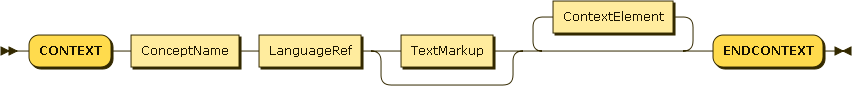
\includegraphics[resolution=120,max size={\textwidth}{\textheight}]{Figures/Ebnf/Context}
  \caption*{\texttt{Context \small::=  `CONTEXT' ConceptName LanguageRef TextMarkup? ContextElement* `ENDCONTEXT'}}
  \label{fig:ebnf-Context}
 \end{figure}

 \begin{figure}[H]
  \centering
  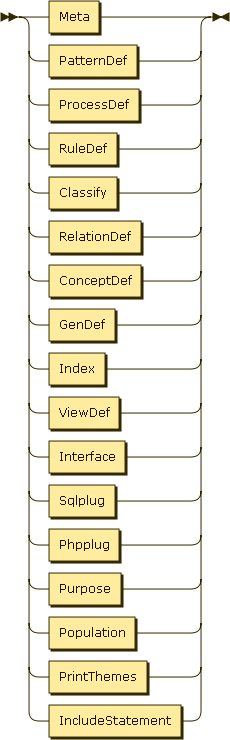
\includegraphics[resolution=120,max size={\textwidth}{\textheight}]{Figures/Ebnf/ContextElement}
  \caption*{\texttt{ContextElement \small::=  Meta | PatternDef | ProcessDef | RuleDef | Classify | RelationDef | ConceptDef | GenDef | Index | ViewDef | Interface | Sqlplug | Phpplug | Purpose | Population | PrintThemes | IncludeStatement}}
  \label{fig:ebnf-ContextElement}
 \end{figure}

 \begin{figure}[H]
  \centering
  
\includegraphics[resolution=120,max size={\textwidth}{\textheight}]{Figures/Ebnf/IncludeStatement}
  \caption*{\texttt{IncludeStatement \small::=  `INCLUDE' String}}
  \label{fig:ebnf-IncludeStatement}
 \end{figure}

 \begin{figure}[H]
  \centering
  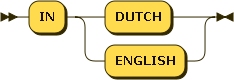
\includegraphics[resolution=120,max size={\textwidth}{\textheight}]{Figures/Ebnf/LanguageRef}
  \caption*{\texttt{LanguageRef \small::=  `IN' (`DUTCH' | `ENGLISH')}}
  \label{fig:ebnf-LanguageRef}
 \end{figure}

 \begin{figure}[H]
  \centering
  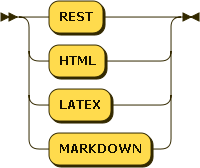
\includegraphics[resolution=120,max size={\textwidth}{\textheight}]{Figures/Ebnf/TextMarkup}
  \caption*{\texttt{TextMarkup \small::=  `REST' | `HTML' | `LATEX' | `MARKDOWN'}}
  \label{fig:ebnf-TextMarkup}
 \end{figure}

 \begin{figure}[H]
  \centering
  
\includegraphics[resolution=120,max size={\textwidth}{\textheight}]{Figures/Ebnf/Meta}
  \caption*{\texttt{Meta \small::=  `META' String String}}
  \label{fig:ebnf-Meta}
 \end{figure}

 \begin{figure}[H]
  \centering
  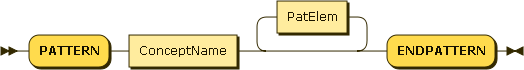
\includegraphics[resolution=120,max size={\textwidth}{\textheight}]{Figures/Ebnf/PatternDef}
  \caption*{\texttt{PatternDef \small::=  `PATTERN' ConceptName PatElem* `ENDPATTERN'}}
  \label{fig:ebnf-PatternDef}
 \end{figure}

 \begin{figure}[H]
  \centering
  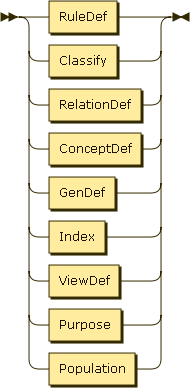
\includegraphics[resolution=120,max size={\textwidth}{\textheight}]{Figures/Ebnf/PatElem}
  \caption*{\texttt{PatElem \small::=  RuleDef | Classify | RelationDef | ConceptDef | GenDef | Index | ViewDef | Purpose | Population}}
  \label{fig:ebnf-PatElem}
 \end{figure}

 \begin{figure}[H]
  \centering
  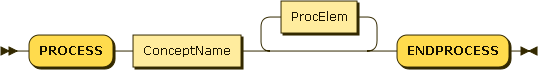
\includegraphics[resolution=120,max size={\textwidth}{\textheight}]{Figures/Ebnf/ProcessDef}
  \caption*{\texttt{ProcessDef \small::=  `PROCESS' ConceptName ProcElem* `ENDPROCESS'}}
  \label{fig:ebnf-ProcessDef}
 \end{figure}

 \begin{figure}[H]
  \centering
  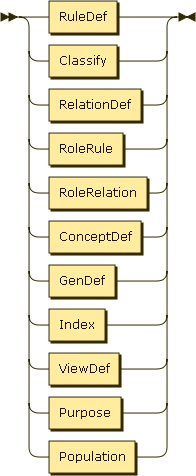
\includegraphics[resolution=120,max size={\textwidth}{\textheight}]{Figures/Ebnf/ProcElem}
  \caption*{\texttt{ProcElem \small::=  RuleDef | Classify | RelationDef | RoleRule | RoleRelation | ConceptDef | GenDef | Index | ViewDef | Purpose | Population}}
  \label{fig:ebnf-ProcElem}
 \end{figure}

 \begin{figure}[H]
  \centering
  
\includegraphics[resolution=120,max size={\textwidth}{\textheight}]{Figures/Ebnf/Classify}
  \caption*{\texttt{Classify \small::=  `CLASSIFY' ConceptRef `IS' Cterm}}
  \label{fig:ebnf-Classify}
 \end{figure}

 \begin{figure}[H]
  \centering
  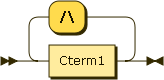
\includegraphics[resolution=120,max size={\textwidth}{\textheight}]{Figures/Ebnf/Cterm}
  \caption*{\texttt{Cterm \small::=  Cterm1 (`/\textbackslash{}' Cterm1)*}}
  \label{fig:ebnf-Cterm}
 \end{figure}

 \begin{figure}[H]
  \centering
  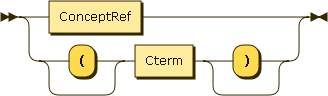
\includegraphics[resolution=120,max size={\textwidth}{\textheight}]{Figures/Ebnf/Cterm1}
  \caption*{\texttt{Cterm1 \small::=  ConceptRef | (`('? Cterm `)'?)}}
  \label{fig:ebnf-Cterm1}
 \end{figure}

 \begin{figure}[H]
  \centering
  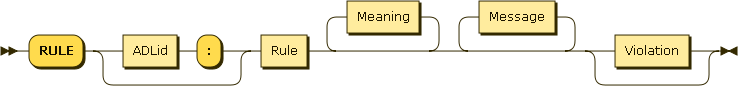
\includegraphics[resolution=120,max size={\textwidth}{\textheight}]{Figures/Ebnf/RuleDef}
  \caption*{\texttt{RuleDef \small::=  `RULE' (ADLid `:')? Rule Meaning* Message* Violation?}}
  \label{fig:ebnf-RuleDef}
 \end{figure}

 \begin{figure}[H]
  \centering
  
\includegraphics[resolution=120,max size={\textwidth}{\textheight}]{Figures/Ebnf/Violation}
  \caption*{\texttt{Violation \small::=  `VIOLATION' PairView}}
  \label{fig:ebnf-Violation}
 \end{figure}

 \begin{figure}[H]
  \centering
  
\includegraphics[resolution=120,max size={\textwidth}{\textheight}]{Figures/Ebnf/PairView}
  \caption*{\texttt{PairView \small::=  `(' PairViewSegmentList `)'}}
  \label{fig:ebnf-PairView}
 \end{figure}

 \begin{figure}[H]
  \centering
  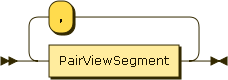
\includegraphics[resolution=120,max size={\textwidth}{\textheight}]{Figures/Ebnf/PairViewSegmentList}
  \caption*{\texttt{PairViewSegmentList \small::=  PairViewSegment (`,' PairViewSegment)*}}
  \label{fig:ebnf-PairViewSegmentList}
 \end{figure}

 \begin{figure}[H]
  \centering
  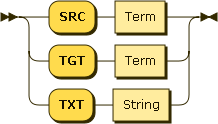
\includegraphics[resolution=120,max size={\textwidth}{\textheight}]{Figures/Ebnf/PairViewSegment}
  \caption*{\texttt{PairViewSegment \small::=  `SRC' Term | `TGT' Term | `TXT' String}}
  \label{fig:ebnf-PairViewSegment}
 \end{figure}

 \begin{figure}[H]
  \centering
  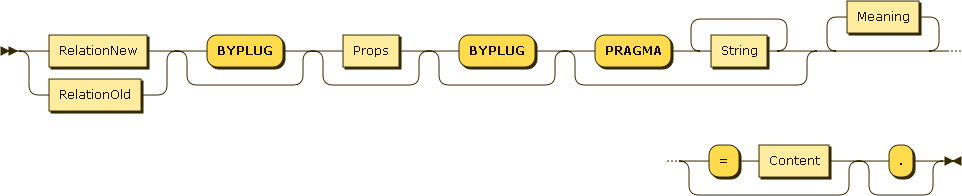
\includegraphics[resolution=120,max size={\textwidth}{\textheight}]{Figures/Ebnf/RelationDef}
  \caption*{\texttt{RelationDef \small::=  (RelationNew | RelationOld) `BYPLUG'? Props? `BYPLUG'? (`PRAGMA' String+)? Meaning* (`=' Content)? `.'?}}
  \label{fig:ebnf-RelationDef}
 \end{figure}

 \begin{figure}[H]
  \centering
  
\includegraphics[resolution=120,max size={\textwidth}{\textheight}]{Figures/Ebnf/RelationNew}
  \caption*{\texttt{RelationNew \small::=  `RELATION' Varid Sign}}
  \label{fig:ebnf-RelationNew}
 \end{figure}

 \begin{figure}[H]
  \centering
  
\includegraphics[resolution=120,max size={\textwidth}{\textheight}]{Figures/Ebnf/RelationOld}
  \caption*{\texttt{RelationOld \small::=  Varid `::' ConceptRef Fun ConceptRef}}
  \label{fig:ebnf-RelationOld}
 \end{figure}

 \begin{figure}[H]
  \centering
  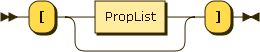
\includegraphics[resolution=120,max size={\textwidth}{\textheight}]{Figures/Ebnf/Props}
  \caption*{\texttt{Props \small::=  `[' PropList? `]'}}
  \label{fig:ebnf-Props}
 \end{figure}

 \begin{figure}[H]
  \centering
  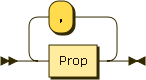
\includegraphics[resolution=120,max size={\textwidth}{\textheight}]{Figures/Ebnf/PropList}
  \caption*{\texttt{PropList \small::=  Prop (`,' Prop)*}}
  \label{fig:ebnf-PropList}
 \end{figure}

 \begin{figure}[H]
  \centering
  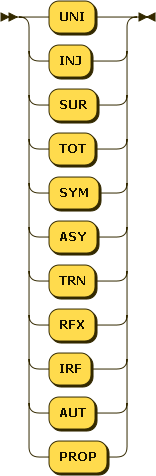
\includegraphics[resolution=120,max size={\textwidth}{\textheight}]{Figures/Ebnf/Prop}
  \caption*{\texttt{Prop \small::=  `UNI' | `INJ' | `SUR' | `TOT' | `SYM' | `ASY' | `TRN' | `RFX' | `IRF' | `AUT' | `PROP'}}
  \label{fig:ebnf-Prop}
 \end{figure}

 \begin{figure}[H]
  \centering
  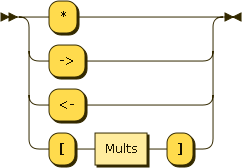
\includegraphics[resolution=120,max size={\textwidth}{\textheight}]{Figures/Ebnf/Fun}
  \caption*{\texttt{Fun \small::=  `*' | `->' | `<-' | `[' Mults `]'}}
  \label{fig:ebnf-Fun}
 \end{figure}

 \begin{figure}[H]
  \centering
  
\includegraphics[resolution=120,max size={\textwidth}{\textheight}]{Figures/Ebnf/Mults}
  \caption*{\texttt{Mults \small::=  Mult `-' Mult}}
  \label{fig:ebnf-Mults}
 \end{figure}

 \begin{figure}[H]
  \centering
  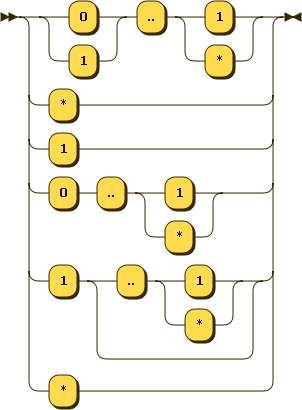
\includegraphics[resolution=120,max size={\textwidth}{\textheight}]{Figures/Ebnf/Mult}
  \caption*{\texttt{Mult \small::=  (`0' | `1') `..' (`1' | `*') | `*' | `1'}}
  \label{fig:ebnf-Mult}
 \end{figure}

 \begin{figure}[H]
  \centering
  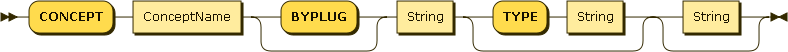
\includegraphics[resolution=120,max size={\textwidth}{\textheight}]{Figures/Ebnf/ConceptDef}
  \caption*{\texttt{ConceptDef \small::=  `CONCEPT' ConceptName `BYPLUG'? String (`TYPE' String)? String?}}
  \label{fig:ebnf-ConceptDef}
 \end{figure}

 \begin{figure}[H]
  \centering
  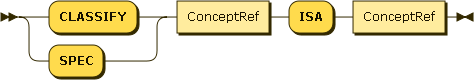
\includegraphics[resolution=120,max size={\textwidth}{\textheight}]{Figures/Ebnf/GenDef}
  \caption*{\texttt{GenDef \small::=  (`CLASSIFY' | `SPEC') ConceptRef `ISA' ConceptRef}}
  \label{fig:ebnf-GenDef}
 \end{figure}

 \begin{figure}[H]
  \centering
  
\includegraphics[resolution=120,max size={\textwidth}{\textheight}]{Figures/Ebnf/Index}
  \caption*{\texttt{Index \small::=  `IDENT' Label ConceptRefPos `(' IndSegmentList `)'}}
  \label{fig:ebnf-Index}
 \end{figure}

 \begin{figure}[H]
  \centering
  
\includegraphics[resolution=120,max size={\textwidth}{\textheight}]{Figures/Ebnf/IndSegmentList}
  \caption*{\texttt{IndSegmentList \small::=  IndSegment (`,' IndSegment)}}
  \label{fig:ebnf-IndSegmentList}
 \end{figure}

 \begin{figure}[H]
  \centering
  
\includegraphics[resolution=120,max size={\textwidth}{\textheight}]{Figures/Ebnf/IndSegment}
  \caption*{\texttt{IndSegment \small::=  IndAtt}}
  \label{fig:ebnf-IndSegment}
 \end{figure}

 \begin{figure}[H]
  \centering
  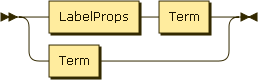
\includegraphics[resolution=120,max size={\textwidth}{\textheight}]{Figures/Ebnf/IndAtt}
  \caption*{\texttt{IndAtt \small::=  LabelProps Term | Term}}
  \label{fig:ebnf-IndAtt}
 \end{figure}

 \begin{figure}[H]
  \centering
  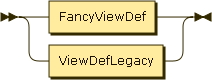
\includegraphics[resolution=120,max size={\textwidth}{\textheight}]{Figures/Ebnf/ViewDef}
  \caption*{\texttt{ViewDef \small::=  FancyViewDef | ViewDefLegacy}}
  \label{fig:ebnf-ViewDef}
 \end{figure}

 \begin{figure}[H]
  \centering
  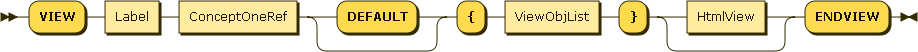
\includegraphics[resolution=120,max size={\textwidth}{\textheight}]{Figures/Ebnf/FancyViewDef}
  \caption*{\texttt{FancyViewDef \small::=  `VIEW' pLabel ConceptOneRefPos `DEFAULT'? `\{' ViewObjList `\}' HtmlView? `ENDVIEW'}}
  \label{fig:ebnf-FancyViewDef}
 \end{figure}

 \begin{figure}[H]
  \centering
  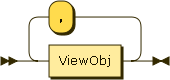
\includegraphics[resolution=120,max size={\textwidth}{\textheight}]{Figures/Ebnf/ViewObjList}
  \caption*{\texttt{ViewObjList \small::=  ViewObj (`,' ViewObj)*}}
  \label{fig:ebnf-ViewObjList}
 \end{figure}

 \begin{figure}[H]
  \centering
  
\includegraphics[resolution=120,max size={\textwidth}{\textheight}]{Figures/Ebnf/ViewObj}
  \caption*{\texttt{ViewObj \small::=  Label Term}}
  \label{fig:ebnf-ViewObj}
 \end{figure}

 \begin{figure}[H]
  \centering
  
\includegraphics[resolution=120,max size={\textwidth}{\textheight}]{Figures/Ebnf/HtmlView}
  \caption*{\texttt{HtmlView \small::=  `HTML' `TEMPLATE' String}}
  \label{fig:ebnf-HtmlView}
 \end{figure}

 \begin{figure}[H]
  \centering
  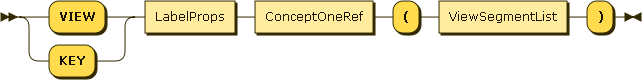
\includegraphics[resolution=120,max size={\textwidth}{\textheight}]{Figures/Ebnf/ViewDefLegacy}
  \caption*{\texttt{ViewDefLegacy \small::=  (`VIEW' | `KEY') LabelProps ConceptOneRefPos `(' ViewSegmentList `)'}}
  \label{fig:ebnf-ViewDefLegacy}
 \end{figure}

 \begin{figure}[H]
  \centering
  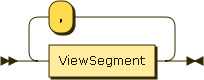
\includegraphics[resolution=120,max size={\textwidth}{\textheight}]{Figures/Ebnf/ViewSegmentList}
  \caption*{\texttt{ViewSegmentList \small::=  ViewSegment (`,' ViewSegment)*}}
  \label{fig:ebnf-ViewSegmentList}
 \end{figure}

 \begin{figure}[H]
  \centering
  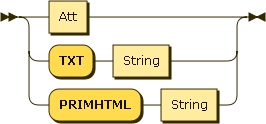
\includegraphics[resolution=120,max size={\textwidth}{\textheight}]{Figures/Ebnf/ViewSegment}
  \caption*{\texttt{ViewSegment \small::=  ViewAtt | `TXT' String | `PRIMHTML' String}}
  \label{fig:ebnf-ViewSegment}
 \end{figure}

 \begin{figure}[H]
  \centering
  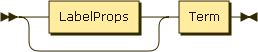
\includegraphics[resolution=120,max size={\textwidth}{\textheight}]{Figures/Ebnf/ViewAtt}
  \caption*{\texttt{ViewAtt \small::=  LabelProps? Term}}
  \label{fig:ebnf-ViewAtt}
 \end{figure}

 \begin{figure}[H]
  \centering
  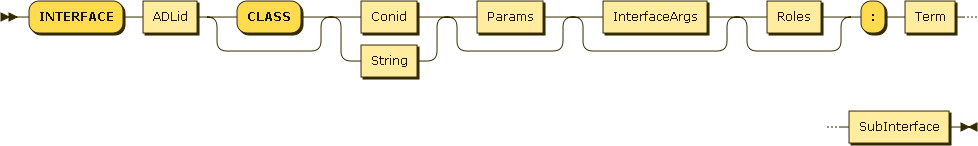
\includegraphics[resolution=120,max size={\textwidth}{\textheight}]{Figures/Ebnf/Interface}
  \caption*{\texttt{Interface \small::=  `INTERFACE' ADLid `CLASS'? (Conid | String) Params? InterfaceArgs? Roles? `:' Term SubInterface}}
  \label{fig:ebnf-Interface}
 \end{figure}

 \begin{figure}[H]
  \centering
  
\includegraphics[resolution=120,max size={\textwidth}{\textheight}]{Figures/Ebnf/Params}
  \caption*{\texttt{Params \small::=  `(' NamedRel `)'}}
  \label{fig:ebnf-Params}
 \end{figure}

 \begin{figure}[H]
  \centering
  
\includegraphics[resolution=120,max size={\textwidth}{\textheight}]{Figures/Ebnf/InterfaceArgs}
  \caption*{\texttt{InterfaceArgs \small::=  `\{' ADLidListList `\}'}}
  \label{fig:ebnf-InterfaceArgs}
 \end{figure}

 \begin{figure}[H]
  \centering
  \includegraphics[resolution=120,max size={\textwidth}{\textheight}]{Figures/Ebnf/Roles}
  \caption*{\texttt{Roles \small::=  `FOR' RoleList}}
  \label{fig:ebnf-Roles}
 \end{figure}

 \begin{figure}[H]
  \centering
  \includegraphics[resolution=120,max size={\textwidth}{\textheight}]{Figures/Ebnf/SubInterface}
  \caption*{\texttt{SubInterface \small::=  (`BOX' (`<' Conid `>')? | `ROWS' | `COLS') Box | `INTERFACE' ADLid}}
  \label{fig:ebnf-SubInterface}
 \end{figure}

 \begin{figure}[H]
  \centering
  \includegraphics[resolution=120,max size={\textwidth}{\textheight}]{Figures/Ebnf/ObjDef}
  \caption*{\texttt{ObjDef \small::=  LabelProps Term (`<' Conid `>')? SubInterface?}}
  \label{fig:ebnf-ObjDef}
 \end{figure}

 \begin{figure}[H]
  \centering
  \includegraphics[resolution=120,max size={\textwidth}{\textheight}]{Figures/Ebnf/ObjDefList}
  \caption*{\texttt{ObjDefList \small::=  ObjDef (`,' ObjDef)*}}
  \label{fig:ebnf-ObjDefList}
 \end{figure}

 \begin{figure}[H]
  \centering
  \includegraphics[resolution=120,max size={\textwidth}{\textheight}]{Figures/Ebnf/Box}
  \caption*{\texttt{Box \small::=  `[' ObjDefList `]'}}
  \label{fig:ebnf-Box}
 \end{figure}

 \begin{figure}[H]
  \centering
  \includegraphics[resolution=120,max size={\textwidth}{\textheight}]{Figures/Ebnf/Sqlplug}
  \caption*{\texttt{Sqlplug \small::=  `SQLPLUG' ObjDef}}
  \label{fig:ebnf-Sqlplug}
 \end{figure}

 \begin{figure}[H]
  \centering
  \includegraphics[resolution=120,max size={\textwidth}{\textheight}]{Figures/Ebnf/Phpplug}
  \caption*{\texttt{Phpplug \small::=  `PHPPLUG' ObjDef}}
  \label{fig:ebnf-Phpplug}
 \end{figure}

 \begin{figure}[H]
  \centering
  \includegraphics[resolution=120,max size={\textwidth}{\textheight}]{Figures/Ebnf/Purpose}
  \caption*{\texttt{Purpose \small::=  `PURPOSE' Ref2Obj LanguageRef? TextMarkup? (`REF' StringListSemi)? Expl}}
  \label{fig:ebnf-Purpose}
 \end{figure}

 \begin{figure}[H]
  \centering
  \includegraphics[resolution=120,max size={\textwidth}{\textheight}]{Figures/Ebnf/Ref2Obj}
  \caption*{\texttt{Ref2Obj \small::=  `CONCEPT' ConceptName | `RELATION' RelSign | `RULE' ADLid | `IDENT' ADLid | `VIEW' ADLid | `PATTERN' ADLid | `PROCESS' ADLid | `INTERFACE' ADLid | `CONTEXT' ADLid}}
  \label{fig:ebnf-Ref2Obj}
 \end{figure}

 \begin{figure}[H]
  \centering
  \includegraphics[resolution=120,max size={\textwidth}{\textheight}]{Figures/Ebnf/Population}
  \caption*{\texttt{Population \small::=  `POPULATION' NamedRel `CONTAINS' Content | `POPULATION' ConceptName `CONTAINS' `[' ValueList `]'}}
  \label{fig:ebnf-Population}
 \end{figure}

 \begin{figure}[H]
  \centering
  \includegraphics[resolution=120,max size={\textwidth}{\textheight}]{Figures/Ebnf/RoleRelation}
  \caption*{\texttt{RoleRelation \small::=  `ROLE' RoleList `EDITS' NamedRelList}}
  \label{fig:ebnf-RoleRelation}
 \end{figure}

 \begin{figure}[H]
  \centering
  \includegraphics[resolution=120,max size={\textwidth}{\textheight}]{Figures/Ebnf/RoleRule}
  \caption*{\texttt{RoleRule \small::=  `ROLE' RoleList `MAINTAINS' ADLidList}}
  \label{fig:ebnf-RoleRule}
 \end{figure}

 \begin{figure}[H]
  \centering
  \includegraphics[resolution=120,max size={\textwidth}{\textheight}]{Figures/Ebnf/Role}
  \caption*{\texttt{Role \small::=  ADLid}}
  \label{fig:ebnf-Role}
 \end{figure}

 \begin{figure}[H]
  \centering
  \includegraphics[resolution=120,max size={\textwidth}{\textheight}]{Figures/Ebnf/RoleList}
  \caption*{\texttt{RoleList \small::=  Role (`,' Role)*}}
  \label{fig:ebnf-RoleList}
 \end{figure}

 \begin{figure}[H]
  \centering
  \includegraphics[resolution=120,max size={\textwidth}{\textheight}]{Figures/Ebnf/PrintThemes}
  \caption*{\texttt{PrintThemes \small::=  `THEMES' ConceptNameList}}
  \label{fig:ebnf-PrintThemes}
 \end{figure}

 \begin{figure}[H]
  \centering
  \includegraphics[resolution=120,max size={\textwidth}{\textheight}]{Figures/Ebnf/Meaning}
  \caption*{\texttt{Meaning \small::=  `MEANING' LanguageRef? TextMarkup? (String | Expl)}}
  \label{fig:ebnf-Meaning}
 \end{figure}

 \begin{figure}[H]
  \centering
  \includegraphics[resolution=120,max size={\textwidth}{\textheight}]{Figures/Ebnf/Message}
  \caption*{\texttt{Message \small::=  `MESSAGE' Markup}}
  \label{fig:ebnf-Message}
 \end{figure}

 \begin{figure}[H]
  \centering
  \includegraphics[resolution=120,max size={\textwidth}{\textheight}]{Figures/Ebnf/Rule}
  \caption*{\texttt{Rule \small::=  Term (`=' Term | `|-' Term)?}}
  \label{fig:ebnf-Rule}
 \end{figure}

 \begin{figure}[H]
  \centering
  \includegraphics[resolution=120,max size={\textwidth}{\textheight}]{Figures/Ebnf/Term}
  \caption*{\texttt{Term \small::=  Trm2 ((`/\textbackslash{}' Trm2)+ | (`\textbackslash{}/' Trm2)+)?}}
  \label{fig:ebnf-Term}
 \end{figure}

 \begin{figure}[H]
  \centering
  \includegraphics[resolution=120,max size={\textwidth}{\textheight}]{Figures/Ebnf/Trm2}
  \caption*{\texttt{Trm2 \small::=  Trm3 (`-' Trm3)?}}
  \label{fig:ebnf-Trm2}
 \end{figure}

 \begin{figure}[H]
  \centering
  \includegraphics[resolution=120,max size={\textwidth}{\textheight}]{Figures/Ebnf/Trm3}
  \caption*{\texttt{Trm3 \small::=  Trm4 (`/' Trm4 | `\textbackslash{}' Trm4 | `<>' Trm4)?}}
  \label{fig:ebnf-Trm3}
 \end{figure}

 \begin{figure}[H]
  \centering
  \includegraphics[resolution=120,max size={\textwidth}{\textheight}]{Figures/Ebnf/Trm4}
  \caption*{\texttt{Trm4 \small::=  Trm5 ((`;' Trm5)+ | (`!' Trm5)+ | (`\#' Trm5)+)?}}
  \label{fig:ebnf-Trm4}
 \end{figure}

 \begin{figure}[H]
  \centering
  \includegraphics[resolution=120,max size={\textwidth}{\textheight}]{Figures/Ebnf/Trm5}
  \caption*{\texttt{Trm5 \small::=  `-'* Trm6 (`~' | `*' | `+')*}}
  \label{fig:ebnf-Trm5}
 \end{figure}

 \begin{figure}[H]
  \centering
  \includegraphics[resolution=120,max size={\textwidth}{\textheight}]{Figures/Ebnf/Trm6}
  \caption*{\texttt{Trm6 \small::=  RelationRef | `(' Term `)'}}
  \label{fig:ebnf-Trm6}
 \end{figure}

 \begin{figure}[H]
  \centering
  \includegraphics[resolution=120,max size={\textwidth}{\textheight}]{Figures/Ebnf/RelationRef}
  \caption*{\texttt{RelationRef \small::=  RelSign | `I' (`[' ConceptOneRef `]')? | `V' Sign? | Atom (`[' ConceptOneRef `]')?}}
  \label{fig:ebnf-RelationRef}
 \end{figure}

 \begin{figure}[H]
  \centering
  \includegraphics[resolution=120,max size={\textwidth}{\textheight}]{Figures/Ebnf/NamedRelList}
  \caption*{\texttt{NamedRelList \small::=  NamedRel (`,' NamedRel)*}}
  \label{fig:ebnf-NamedRelList}
 \end{figure}

 \begin{figure}[H]
  \centering
  \includegraphics[resolution=120,max size={\textwidth}{\textheight}]{Figures/Ebnf/NamedRel}
  \caption*{\texttt{NamedRel \small::=  Varid Sign?}}
  \label{fig:ebnf-NamedRel}
 \end{figure}

 \begin{figure}[H]
  \centering
  \includegraphics[resolution=120,max size={\textwidth}{\textheight}]{Figures/Ebnf/Sign}
  \caption*{\texttt{Sign \small::=  `[' ConceptOneRef (`*' ConceptOneRef)? `]'}}
  \label{fig:ebnf-Sign}
 \end{figure}

 \begin{figure}[H]
  \centering
  \includegraphics[resolution=120,max size={\textwidth}{\textheight}]{Figures/Ebnf/ConceptName}
  \caption*{\texttt{ConceptName \small::=  Conid | String}}
  \label{fig:ebnf-ConceptName}
 \end{figure}

 \begin{figure}[H]
  \centering
  \includegraphics[resolution=120,max size={\textwidth}{\textheight}]{Figures/Ebnf/ConceptNameList}
  \caption*{\texttt{ConceptNameList \small::=  ConceptName (`,' ConceptName)}}
  \label{fig:ebnf-ConceptNameList}
 \end{figure}

 \begin{figure}[H]
  \centering
  \includegraphics[resolution=120,max size={\textwidth}{\textheight}]{Figures/Ebnf/ConceptRef}
  \caption*{\texttt{ConceptRef \small::=  ConceptName}}
  \label{fig:ebnf-ConceptRef}
 \end{figure}

 \begin{figure}[H]
  \centering
  \includegraphics[resolution=120,max size={\textwidth}{\textheight}]{Figures/Ebnf/ConceptOneRef}
  \caption*{\texttt{ConceptOneRef \small::=  `ONE' | ConceptRef}}
  \label{fig:ebnf-ConceptOneRef}
 \end{figure}

 \begin{figure}[H]
  \centering
  \includegraphics[resolution=120,max size={\textwidth}{\textheight}]{Figures/Ebnf/LabelProps}
  \caption*{\texttt{LabelProps \small::=  ADLid (`\{' ADLidListList `\}')? `:'}}
  \label{fig:ebnf-LabelProps}
 \end{figure}

 \begin{figure}[H]
  \centering
  \includegraphics[resolution=120,max size={\textwidth}{\textheight}]{Figures/Ebnf/Label}
  \caption*{\texttt{Label \small::=  ADLid `:'}}
  \label{fig:ebnf-Label}
 \end{figure}

 \begin{figure}[H]
  \centering
  \includegraphics[resolution=120,max size={\textwidth}{\textheight}]{Figures/Ebnf/Content}
  \caption*{\texttt{Content \small::=  `[' RecordList? `]' | `[' RecordObsList? `]'}}
  \label{fig:ebnf-Content}
 \end{figure}

 \begin{figure}[H]
  \centering
  \includegraphics[resolution=120,max size={\textwidth}{\textheight}]{Figures/Ebnf/RecordList}
  \caption*{\texttt{RecordList \small::=  Record (`,' Record)*}}
  \label{fig:ebnf-RecordList}
 \end{figure}

 \begin{figure}[H]
  \centering
  \includegraphics[resolution=120,max size={\textwidth}{\textheight}]{Figures/Ebnf/Record}
  \caption*{\texttt{Record \small::=  String `*' String}}
  \label{fig:ebnf-Record}
 \end{figure}

 \begin{figure}[H]
  \centering
  \includegraphics[resolution=120,max size={\textwidth}{\textheight}]{Figures/Ebnf/RecordObsList}
  \caption*{\texttt{RecordObsList \small::=  RecordObsList (`;' RecordObsList)}}
  \label{fig:ebnf-RecordObsList}
 \end{figure}

 \begin{figure}[H]
  \centering
  \includegraphics[resolution=120,max size={\textwidth}{\textheight}]{Figures/Ebnf/RecordObs}
  \caption*{\texttt{RecordObs \small::=  `(' String `,' String `)'}}
  \label{fig:ebnf-RecordObs}
 \end{figure}

 \begin{figure}[H]
  \centering
  \includegraphics[resolution=120,max size={\textwidth}{\textheight}]{Figures/Ebnf/ADLid}
  \caption*{\texttt{ADLid \small::=  Varid | Conid | String}}
  \label{fig:ebnf-ADLid}
 \end{figure}

 \begin{figure}[H]
  \centering
  \includegraphics[resolution=120,max size={\textwidth}{\textheight}]{Figures/Ebnf/ADLidList}
  \caption*{\texttt{ADLidList \small::=  ADLid (`,' ADLid)*}}
  \label{fig:ebnf-ADLidList}
 \end{figure}

 \begin{figure}[H]
  \centering
  \includegraphics[resolution=120,max size={\textwidth}{\textheight}]{Figures/Ebnf/ADLidListList}
  \caption*{\texttt{ADLidListList \small::=  ADLid+ (`,' ADLid+)*}}
  \label{fig:ebnf-ADLidListList}
 \end{figure}

 \begin{figure}[H]
  \centering
  \includegraphics[resolution=120,max size={\textwidth}{\textheight}]{Figures/Ebnf/Conid}
  \caption*{\texttt{Conid \small::=  UpperChar (Char | `\_')*}}
  \label{fig:ebnf-Conid}
 \end{figure}

 \begin{figure}[H]
  \centering
  \includegraphics[resolution=120,max size={\textwidth}{\textheight}]{Figures/Ebnf/String}
  \caption*{\texttt{String \small::=  `"' Any* `"'}}
  \label{fig:ebnf-String}
 \end{figure}

 \begin{figure}[H]
  \centering
  \includegraphics[resolution=120,max size={\textwidth}{\textheight}]{Figures/Ebnf/StringListSemi}
  \caption*{\texttt{StringListSemi \small::=  String (`;' String)*}}
  \label{fig:ebnf-StringListSemi}
 \end{figure}

 \begin{figure}[H]
  \centering
  \includegraphics[resolution=120,max size={\textwidth}{\textheight}]{Figures/Ebnf/Expl}
  \caption*{\texttt{Expl \small::=  `\{+' Any* `-\}'}}
  \label{fig:ebnf-Expl}
 \end{figure}

 \begin{figure}[H]
  \centering
  \includegraphics[resolution=120,max size={\textwidth}{\textheight}]{Figures/Ebnf/Varid}
  \caption*{\texttt{Varid \small::=  (LowerChar | `\_') (Char | `\_')*}}
  \label{fig:ebnf-Varid}
 \end{figure}


\newpage
\begin{landscape}

  \section*{Parse Tree}
  \label{app:parse-tree}
  \addcontentsline{toc}{section}{Parse Tree}
  \begin{figure}[htb!]
    \centering
    \includegraphics[width=25.4cm]{Figures/GenParseTree}
    \caption[Diagram of the Ampersand parse tree]{
      Diagram of the Ampersand parse tree. \small
      %Data definitions are depicted in green, constructors are depicted in blue and 
      Connections without an arrow represent the data contructors.
      Connections with an arrow also show the multiplicity in the relationship (i.e. 1 or *) or are stripped to represent an optional relationship.
      }
    \label{fig:parse-tree}
  \end{figure}

\end{landscape}
\newpage
% !TEX root = ../Parsing.tex
\addcontentsline{toc}{section}{References}
\label{sec:bibliography}

\begin{thebibliography}{99}

\bibitem{plan}
	Planning for the project `Useful feedback in the Ampersand parser'\\
	Maarten Baertsoen and Daniel S. C. Schiavini\\
	Version 2.0 -- November 29, 2014\\
	\url{http://git.io/NeHuLg}

\bibitem{heeren-error}
	Top Quality Type Error Messages\\
	Bastiaan Heeren\\
	ISBN 90-393-4005-6, September 20, 2005\\
	\url{http://www.open.ou.nl/bhr/phdthesis}

\bibitem{monadic-parsing}
	Functional pearls -- Monadic Parsing in Haskell\\
	Graham Hutton (University of Nottingham) and Erik Meijer (University of Utrecht)\\
	\url{http://www.cs.nott.ac.uk/~gmh/monparsing.pdf}

\bibitem{convert-ebnf}
	 From EBNF to BNF \\
	 Christoph Zenger\\
	 June 4, 2000\\
	 \url{http://lampwww.epfl.ch/teaching/archive/compilation-ssc/2000/part4/parsing/node3.html}

\bibitem{bnf-ebnf}
	BNF and EBNF: What are they and how do they work?\\
	Lars Marius Garshol\\
	August 22, 2008\\
	\url{http://www.garshol.priv.no/download/text/bnf.html}

\bibitem{parser-examples}
	Haskell Parser Examples\\
	Geoff Hulette\\
	August 22, 2014\\
	\url{https://github.com/ghulette/haskell-parser-examples}

\bibitem{hugs-parser}
	Source code of the Hugs parser\\
	March 25, 2007\\
	\url{https://github.com/fuzxxl/Hugs/blob/master/src/parser.y}

\bibitem{ghc-parser}
	GHC: The Parser\\
	December 1, 2014\\
	\url{https://ghc.haskell.org/trac/ghc/wiki/Commentary/Compiler/Parser}
	%\url{https://ghc.haskell.org/trac/ghc/browser/ghc/compiler/parser/Parser.y}
	%https://www.haskell.org/pipermail/haskell-cafe/2013-August/109557.html

\bibitem{helium-parser}
	Helium, for Learning Haskell\\
	Bastiaan Heeren, Daan Leijen, Arjan van IJzendoorn\\
	Utrecht University\\
	\url{http://www.open.ou.nl/bhr/heeren-helium.pdf}
	
\bibitem{gcc-c-parser}
	GCC 4.1 Release Series Changes, New Features, and Fixes\\
	\url{https://gcc.gnu.org/gcc-3.4/changes.html}

\bibitem{gcc-cpp-parser}
	GCC 3.4 Release Series Changes, New Features, and Fixes\\
	\url{https://gcc.gnu.org/gcc-4.1/changes.html}
	
\end{thebibliography}

\end{document}